\documentclass[conference]{IEEEtran}

% Paquetes estandar compatibles con Overleaf (pdfLaTeX)
\usepackage[utf8]{inputenc}
\usepackage[T1]{fontenc}
\usepackage[spanish,es-tabla]{babel}
\usepackage{cite}
\usepackage{amsmath,amssymb,amsfonts}
\usepackage{graphicx}
\usepackage{booktabs}
\usepackage{multirow}
\usepackage{url}
\usepackage{xcolor}
\usepackage{hyperref}

% Macro para notas de redaccion (borrar cada \guia{...} cuando escriban su parrafo propio)
\newcommand{\guia}[1]{\textcolor{blue}{\textit{[GUIA DE REDACCION: #1]}}}

\begin{document}

\title{Detección y Segmentación de Material Combustible Forestal mediante Imágenes Aéreas Multiespectrales: Comparativa entre Aprendizaje Clásico y Deep Learning}

\author{
\IEEEauthorblockN{Roberto Flores Benítez\IEEEauthorrefmark{1} y Jorge Luis Venegas Segura\IEEEauthorrefmark{2}}
\IEEEauthorblockA{
Facultad de Ingeniería, Universidad Autónoma del Estado de México (UAEMéx)\\
Toluca, Estado de México, México\\
Correos: \IEEEauthorrefmark{1}robertoflores2925@gmail.com, \IEEEauthorrefmark{2}[correo\_jorge@uaemex.mx]
}
}

\maketitle

% =========================================================================
% RESUMEN
% =========================================================================
\begin{abstract}
\guia{Redacta aquí 1 párrafo propio de 150--200 palabras resumiendo:
(1) el problema de detección temprana de combustible forestal seco para prevención de incendios;
(2) el dataset multitemporal (60 capturas 2025--2026 con dron DJI Mavic 3 Multispectral, 3 clases: vegetacion\_seca, vegetacion\_sana y suelo\_desnudo);
(3) la metodología (calibración radiométrica, corregistro SIFT+RANSAC, extracción HOG vs. multiespectral+color, partición espacial sin fuga y entrenamiento de KNN, Random Forest, SVM y YOLO11n-seg);
(4) los resultados clave: en anotaciones 100\% manuales, pasar de solo HOG (45.6\%--55.9\% F1-macro) a rasgos multiespectrales+color elevó el F1-macro a 92.5\%--97.9\%, mientras que YOLO11n-seg logró 93.98\% de exactitud a nivel píxel y 66.55\% de mIoU usando únicamente RGB en ~29.4 ms por parche en CPU.}
\end{abstract}

\begin{IEEEkeywords}
Visión artificial, imágenes multiespectrales, prevención de incendios forestales, NDVI, KNN, Random Forest, SVM, YOLO11-seg.
\end{IEEEkeywords}

% =========================================================================
% I. INTRODUCCION
% =========================================================================
\section{Introducción}

\guia{Párrafo 1 (Contexto y problema, ~100 palabras): Explica con tus palabras el impacto de los incendios forestales, por qué identificar vegetación seca (árboles secos, ramas y hojarasca) es crítico para prevenir ignición y propagación, y las limitaciones de la inspección manual en campo.}

\guia{Párrafo 2 (Brecha técnica, ~100 palabras): Explica que las imágenes RGB convencionales o en escala de grises presentan confusión visual entre vegetación seca, sombras y suelo, mientras que las cámaras multiespectrales en drones (bandas Red-Edge y NIR) capturan la salud clorofílica real de la vegetación \cite{rouse1974ndvi,gitelson1997ndre}.}

\guia{Párrafo 3 (Objetivo y contribuciones, ~90 palabras): Presenta el objetivo del estudio y enumera tus 3 aportes principales:
(a) pipeline de calibración radiométrica y alineación multiespectral SIFT+RANSAC con partición espacial sin fuga de datos;
(b) evaluación comparativa de KNN, Random Forest y SVM comparando solo HOG frente a rasgos multiespectrales+color sobre anotaciones 100\% manuales;
(c) segmentación semántica solo con RGB mediante YOLO11n-seg y generación de mapas aéreos de calor y riesgo de incendio.}

% =========================================================================
% II. MARCO TEORICO Y TRABAJOS RELACIONADOS
% =========================================================================
\section{Marco Teórico}

\guia{Párrafo 1 (Índices espectrales y preprocesamiento, ~100 palabras): Describe brevemente con tus palabras el fundamento físico de NDVI \cite{rouse1974ndvi}, NDRE/GNDVI \cite{gitelson1997ndre} y el índice visible de exceso de verde ExG \cite{woebbecke1995exg}, así como el corregistro de imágenes con SIFT \cite{lowe2004sift} y RANSAC \cite{fischler1981ransac}.}

\guia{Párrafo 2 (Reconocimiento de patrones clásico, ~100 palabras): Explica brevemente qué es el descriptor de gradientes HOG \cite{dalal2005hog}, la segmentación por superpíxeles SLIC \cite{achanta2012slic}, y el principio de los clasificadores supervisados KNN \cite{cover1967knn}, Random Forest \cite{breiman2001rf} y Máquinas de Vectores de Soporte (SVM) \cite{cortes1995svm}.}

\guia{Párrafo 3 (Segmentación con Deep Learning, ~80 palabras): Contrasta los métodos clásicos (que requieren extracción manual de características) con redes convolucionales de una etapa como la familia YOLO \cite{redmon2016yolo,jocher2024yolo11}, capaces de aprender representaciones espaciales y segmentar instancias directamente sobre imágenes RGB.}

% =========================================================================
% III. METODOLOGIA
% =========================================================================
\section{Metodología}

\subsection{Adquisición y Descripción del Dataset}
\guia{Redacta ~90 palabras describiendo el dataset: 60 capturas aéreas nadirales (ángulo de cámara $-89.9^\circ$, altura relativa constante de $\sim 41.2\text{ m}$) adquiridas con un dron DJI Mavic 3 Multispectral con GPS RTK sobre un área forestal de $\sim 288\text{ m} \times 123\text{ m}$ ($\sim 3.5\text{ ha}$). Se realizaron dos campañas sobre los mismos 30 waypoints (desfase mediano de $1.39\text{ m}$): 30 capturas el 29 de marzo de 2025 (luz difusa, irradiancia NIR $\approx 6416$) y 30 capturas el 29 de abril de 2026 (sol directo, irradiancia NIR $\approx 10307$). Cada captura incluye una imagen RGB ($5280 \times 3956\text{ px}$) y cuatro bandas de 16 bits ($2592 \times 1944\text{ px}$): Verde ($560\text{ nm}$), Rojo ($650\text{ nm}$), Red-Edge ($730\text{ nm}$) e Infrarrojo Cercano NIR ($860\text{ nm}$).}

\subsection{Calibración Radiométrica, Corregistro y Tiling}
\guia{Explica con tus palabras (~100 palabras) por qué fue necesario calibrar radiométricamente las bandas (compensando diferencias de sol entre 2025 y 2026 usando nivel de negro, corrección polinomial de viñeteo, ganancia, tiempo de exposición e irradiancia solar del XMP) y corregir la distorsión óptica antes de alinear las lentes físicamente separadas mediante SIFT+RANSAC \cite{lowe2004sift,fischler1981ransac}. Reporta la calidad obtenida en las 60 capturas: correlación mediana NIR--Verde de $0.905$ (rango $0.695$--$0.946$) y MS--RGB de $0.766$ (rango $0.652$--$0.847$). Menciona que se recortó el viñeteo exterior para extraer $1{,}200$ parches RGB limpios de $1024 \times 1024\text{ px}$ (15\% de solape) emparejados con sus mapas espectrales (Fig.~\ref{fig:preproc}).}

Los índices espectrales y cromáticos calculados se definen mediante:
\begin{equation}
\text{NDVI} = \frac{\text{NIR} - R}{\text{NIR} + R}, \qquad
\text{NDRE} = \frac{\text{NIR} - \text{RE}}{\text{NIR} + \text{RE}}
\label{eq:ndvi_ndre}
\end{equation}
\begin{equation}
\text{GNDVI} = \frac{\text{NIR} - G}{\text{NIR} + G}, \qquad
\text{ExG} = \frac{2G - R - B}{R + G + B}
\label{eq:gndvi_exg}
\end{equation}

\begin{figure*}[!t]
\centering
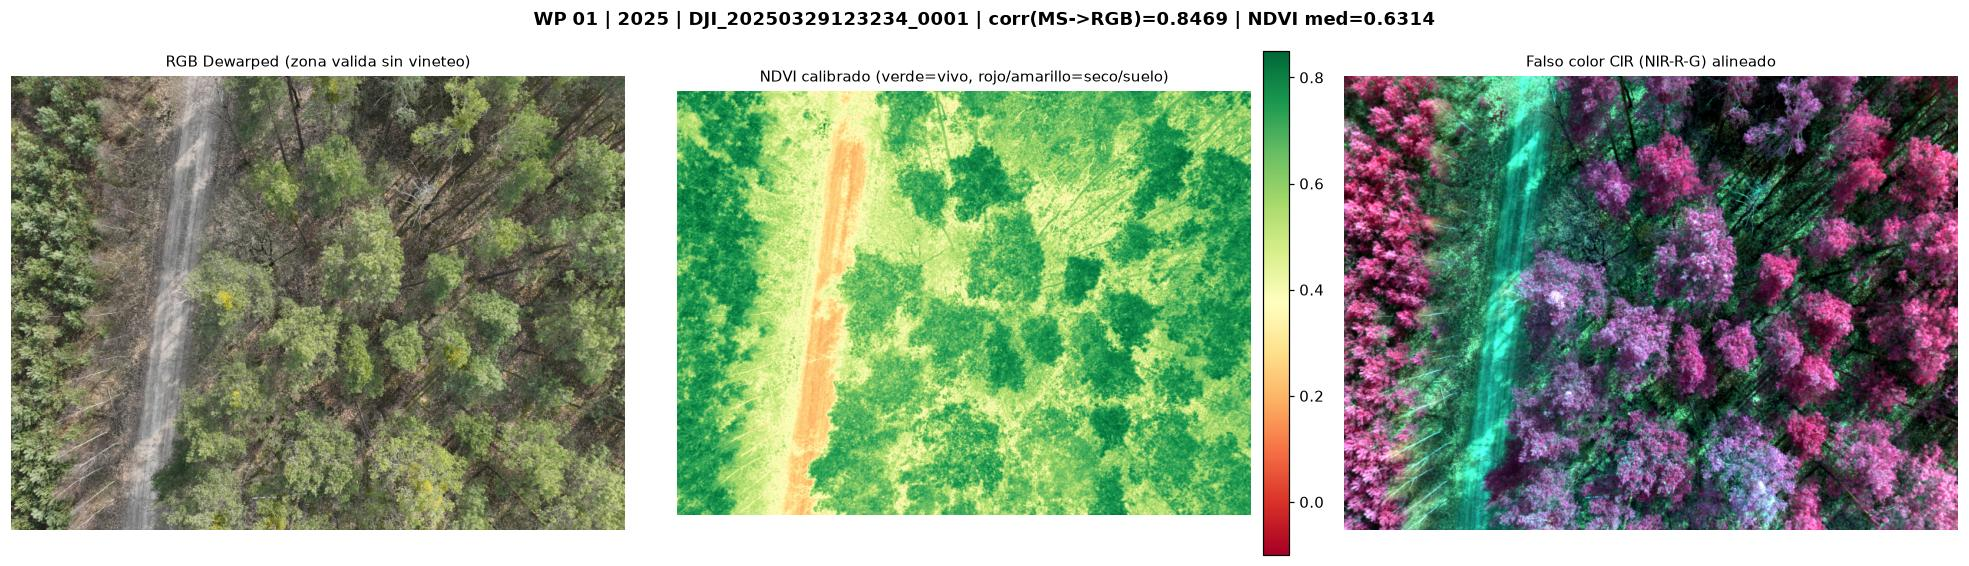
\includegraphics[width=0.96\textwidth]{figuras/fig1_preprocesamiento.jpg}
\caption{Control visual del preprocesamiento multiespectral (Waypoint 01, campaña 2025): imagen RGB corregida sin viñeteo (izquierda), mapa NDVI calibrado (centro) y composición en falso color CIR NIR--R--G corregistrada mediante SIFT+RANSAC (derecha).}
\label{fig:preproc}
\end{figure*}

\subsection{Definición de Clases, Etiquetado y Partición Espacial}
\guia{Explica con tus palabras (~110 palabras) las 3 clases unificadas (\texttt{vegetacion\_seca}, \texttt{vegetacion\_sana} y \texttt{suelo\_desnudo}) y los dos conjuntos de anotaciones en formato LabelMe \cite{wada2016labelme}:
(1) un conjunto de 240 parches ($120$ de 2025 y $120$ de 2026) pre-anotados mediante superpíxeles SLIC \cite{achanta2012slic} con índices espectrales, textura Sobel y jerarquía estricta sin solapes (solape residual medio de $0.31\%$, revisado visualmente en LabelMe), totalizando $1{,}880$ polígonos;
(2) un conjunto independiente de 45 fotografías completas etiquetadas 100\% manualmente en LabelMe ($411$ cajas, de las cuales $307$ quedan dentro de la cobertura multiespectral válida).
Enfatiza la partición espacial estricta por waypoint (21 waypoints entrenamiento, 5 validación y 4 prueba, manteniendo 2025 y 2026 del mismo punto en el mismo subconjunto) para evitar fuga de datos espacial (Tabla~\ref{tab:split}).}

\begin{table}[!t]
\centering
\caption{Distribución espacial del dataset de segmentación (240 parches, 0 waypoints compartidos entre subconjuntos).}
\label{tab:split}
\begin{tabular}{lccccc}
\toprule
\textbf{Subconjunto} & \textbf{WPs} & \textbf{Imágenes} & \textbf{Veg. Seca} & \textbf{Veg. Sana} & \textbf{Suelo} \\
\midrule
Entrenamiento & 21 & 159 & 736 & 331 & 183 \\
Validación    & 5  & 40  & 209 & 72  & 48  \\
Prueba (Test) & 4  & 41  & 185 & 65  & 51  \\
\midrule
\textbf{Total} & \textbf{30} & \textbf{240} & \textbf{1,130} & \textbf{468} & \textbf{282} \\
\bottomrule
\end{tabular}
\end{table}

\subsection{Extracción de Características y Modelos Evaluados}
\guia{Explica con tus palabras (~120 palabras) los dos paradigmas comparados:
(1) \textbf{Modelos clásicos} (KNN, Random Forest con 300 árboles y \texttt{class\_weight=balanced}, y SVM con kernel RBF ajustado en validación) evaluados bajo dos extractores: (a) \emph{Solo HOG} en escala de grises ($128 \times 128$, 9 orientaciones, celdas $8\times8$, bloques $2\times2$, $8{,}100$ características con reducción PCA) y (b) \emph{22 rasgos Multiespectral + Color + Textura} (estadísticos de NDVI, NDRE, GNDVI, ExG, HSV, CIE Lab, gradiente Sobel y área logarítmica).
(2) \textbf{Deep Learning}: red \texttt{YOLO11n-seg} ($2.85\text{ M}$ parámetros) entrenada durante 40 épocas únicamente con imágenes RGB ($512\times512$, optimizador AdamW, rotaciones de $180^\circ$ y volteos para vista cenital). En inferencia sobre fotos completas se utilizó ventana deslizante de $1024\times1024$ con 25\% de solape y ponderación Hann para construir mapas de calor continuos.}

Las métricas de clasificación y segmentación semántica utilizadas fueron Exactitud (Accuracy), F1-Score e Intersección sobre Unión (IoU):
\begin{equation}
\text{F1} = \frac{2 \cdot \text{P} \cdot \text{R}}{\text{P} + \text{R}}, \qquad
\text{IoU} = \frac{\text{TP}}{\text{TP} + \text{FP} + \text{FN}}
\label{eq:f1_iou}
\end{equation}

% =========================================================================
% IV. RESULTADOS Y DISCUSION
% =========================================================================
\section{Resultados y Discusión}

\subsection{Comparativa de Modelos Clásicos en Anotaciones Manuales}
\guia{Analiza con tus palabras (~120 palabras) la Tabla~\ref{tab:clasicos} y la Fig.~\ref{fig:comp_maestra}(A). Destaca el hallazgo principal: al usar únicamente HOG en escala de grises, los tres algoritmos fallan al separar clases espectralmente distintas (F1-macro entre $45.6\%$ y $55.9\%$, llegando a $0.000$ en \texttt{vegetacion\_seca} para KNN). Al incorporar los 22 rasgos multiespectrales y de color, todos los modelos dan un salto de $+36.6$ a $+50.3$ puntos en F1-macro, alcanzando KNN $98.88\%$ de exactitud ($97.91\%$ F1-macro), Random Forest $97.75\%$ ($95.86\%$ F1-macro) y SVM $95.51\%$ ($92.53\%$ F1-macro). Además, resalta la prueba \emph{Zero-Shot} (modelos entrenados en los 240 parches pre-anotados y evaluados sin reentrenar en las anotaciones manuales): Random Forest alcanza $91.01\%$ de exactitud ($85.22\%$ F1-macro), validando la consistencia del etiquetado asistido.}

\begin{table}[!t]
\centering
\caption{Evaluación de modelos clásicos en anotaciones 100\% manuales (split espacial, 307 cajas válidas).}
\label{tab:clasicos}
\resizebox{\columnwidth}{!}{%
\begin{tabular}{llccccc}
\toprule
\textbf{Extractor} & \textbf{Modelo} & \textbf{Acc (\%)} & \textbf{F1-Mac (\%)} & \textbf{F1 Seca} & \textbf{F1 Sana} & \textbf{F1 Suelo} \\
\midrule
\multirow{3}{*}{Solo HOG}
 & KNN & 69.66 & 47.58 & 0.000 & 0.812 & 0.615 \\
 & RF  & 71.91 & 45.64 & 0.533 & 0.836 & 0.000 \\
 & SVM & 75.28 & 55.90 & 0.100 & 0.871 & 0.706 \\
\midrule
\multirow{3}{*}{\shortstack[l]{Multiespectral\\+ Color}}
 & \textbf{KNN} & \textbf{98.88} & \textbf{97.91} & \textbf{0.974} & \textbf{1.000} & \textbf{0.963} \\
 & RF  & 97.75 & 95.86 & 0.947 & 1.000 & 0.929 \\
 & SVM & 95.51 & 92.53 & 0.905 & 0.991 & 0.880 \\
\midrule
\multirow{3}{*}{\shortstack[l]{Zero-Shot\\(Fase3$\to$Man.)}}
 & KNN & 86.52 & 78.32 & 0.727 & 0.956 & 0.667 \\
 & \textbf{RF}  & \textbf{91.01} & \textbf{85.22} & 0.800 & \textbf{0.974} & \textbf{0.783} \\
 & SVM & 86.52 & 80.03 & \textbf{0.824} & 0.911 & 0.667 \\
\bottomrule
\end{tabular}%
}
\end{table}

\begin{figure*}[!t]
\centering
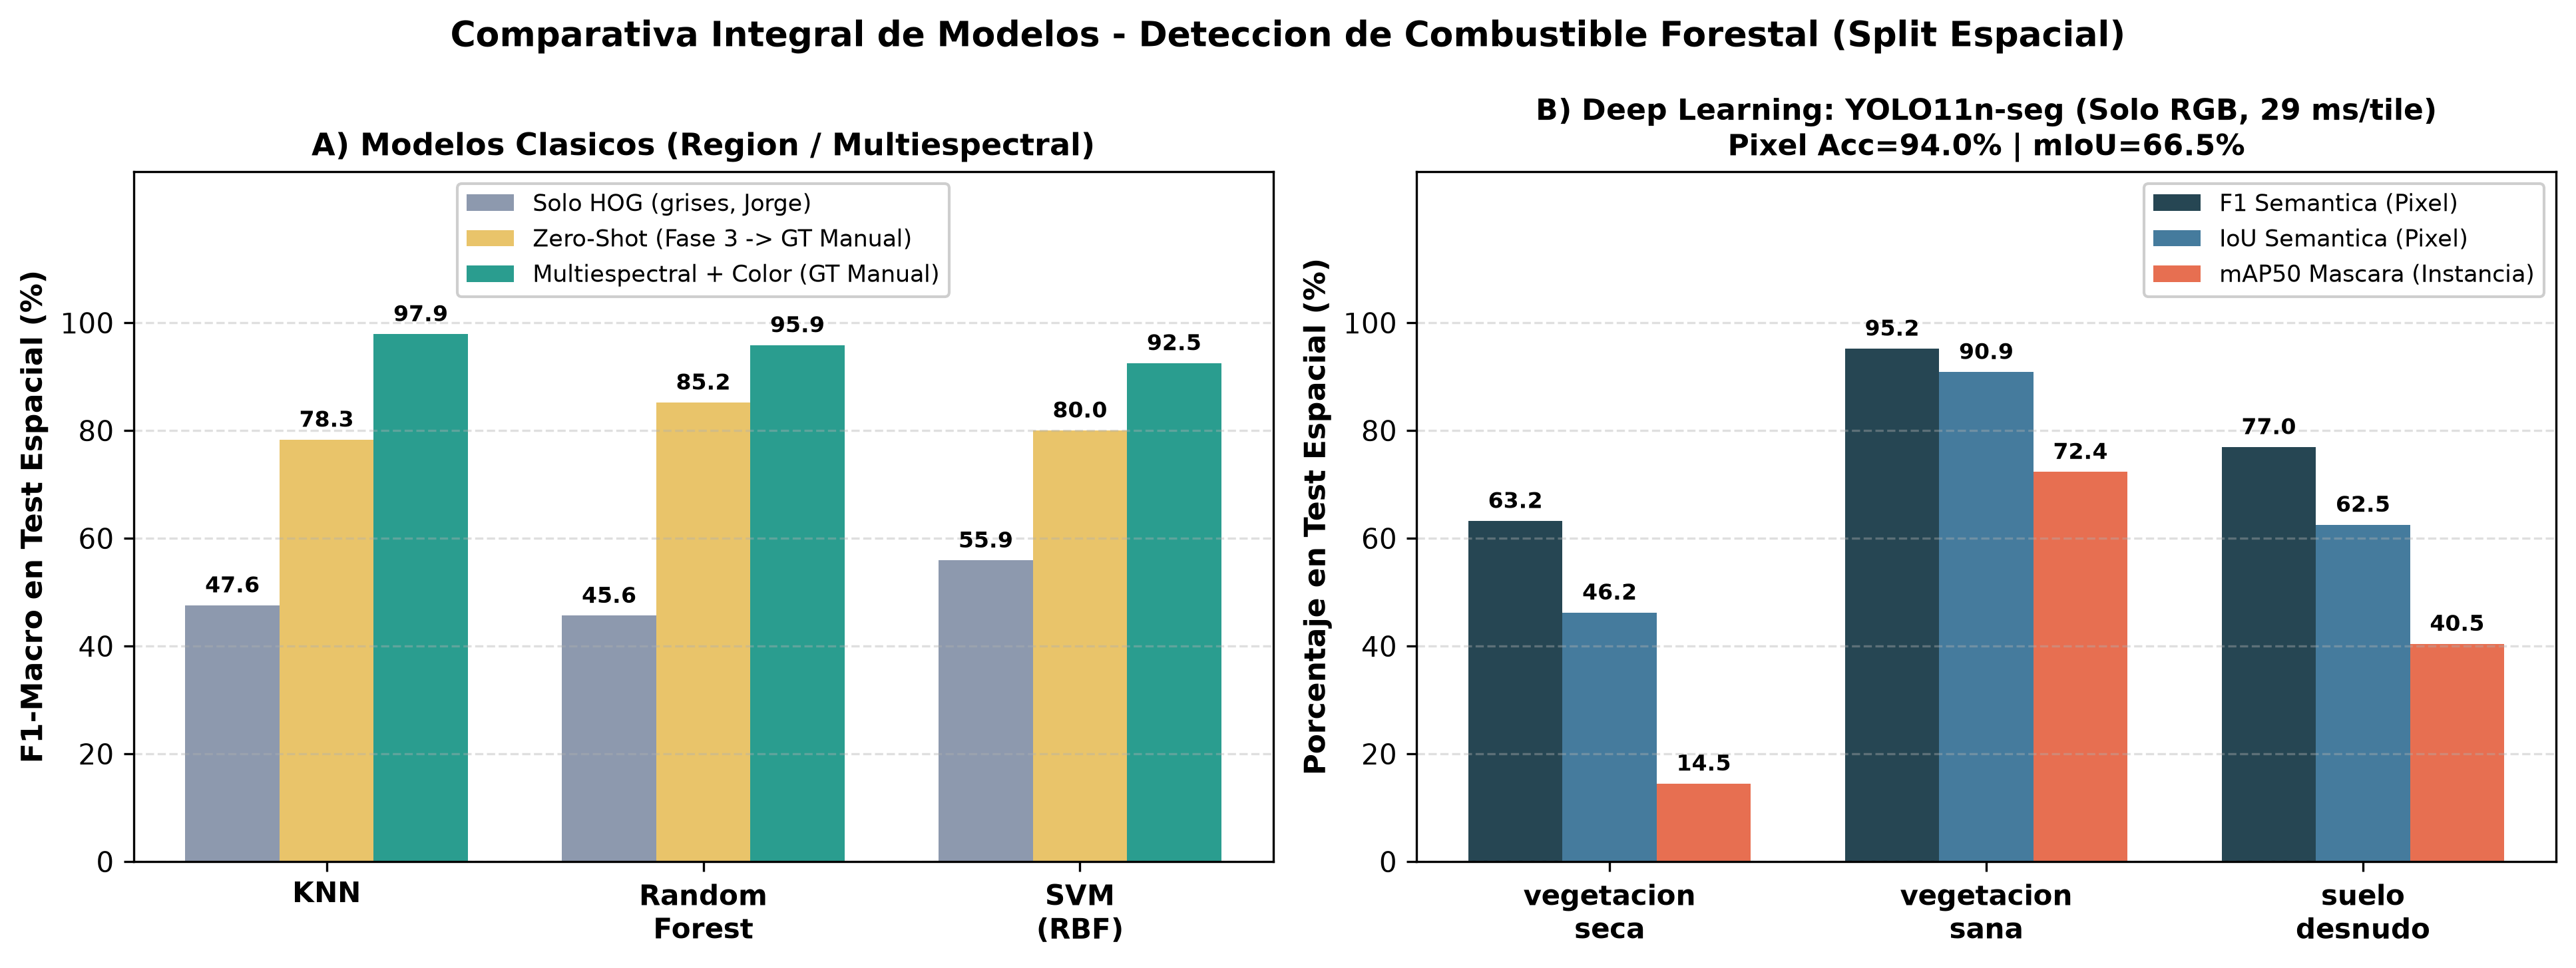
\includegraphics[width=0.96\textwidth]{figuras/fig2_comparativa_maestra.png}
\caption{Comparativa integral en el conjunto de prueba espacial: (A) F1-macro de KNN, Random Forest y SVM con solo HOG, transferencia Zero-Shot y rasgos multiespectrales+color sobre anotaciones manuales; (B) desempeño semántico a nivel píxel e instancia de YOLO11n-seg operando exclusivamente con imágenes RGB.}
\label{fig:comp_maestra}
\end{figure*}

\guia{Párrafo breve (~70 palabras) comentando la Fig.~\ref{fig:imp_rf}: explica cuáles fueron las variables con mayor peso en Random Forest (\texttt{ExG\_mean} $16.6\%$, \texttt{NDVI\_mean} $11.8\%$, \texttt{Lab\_a\_mean} $10.9\%$, \texttt{NDVI\_p90} $8.2\%$, \texttt{GNDVI\_mean} $6.8\%$), señalando que las bandas infrarrojas aportan en conjunto $\sim 35\%$ del poder discriminativo.}

\begin{figure}[!t]
\centering
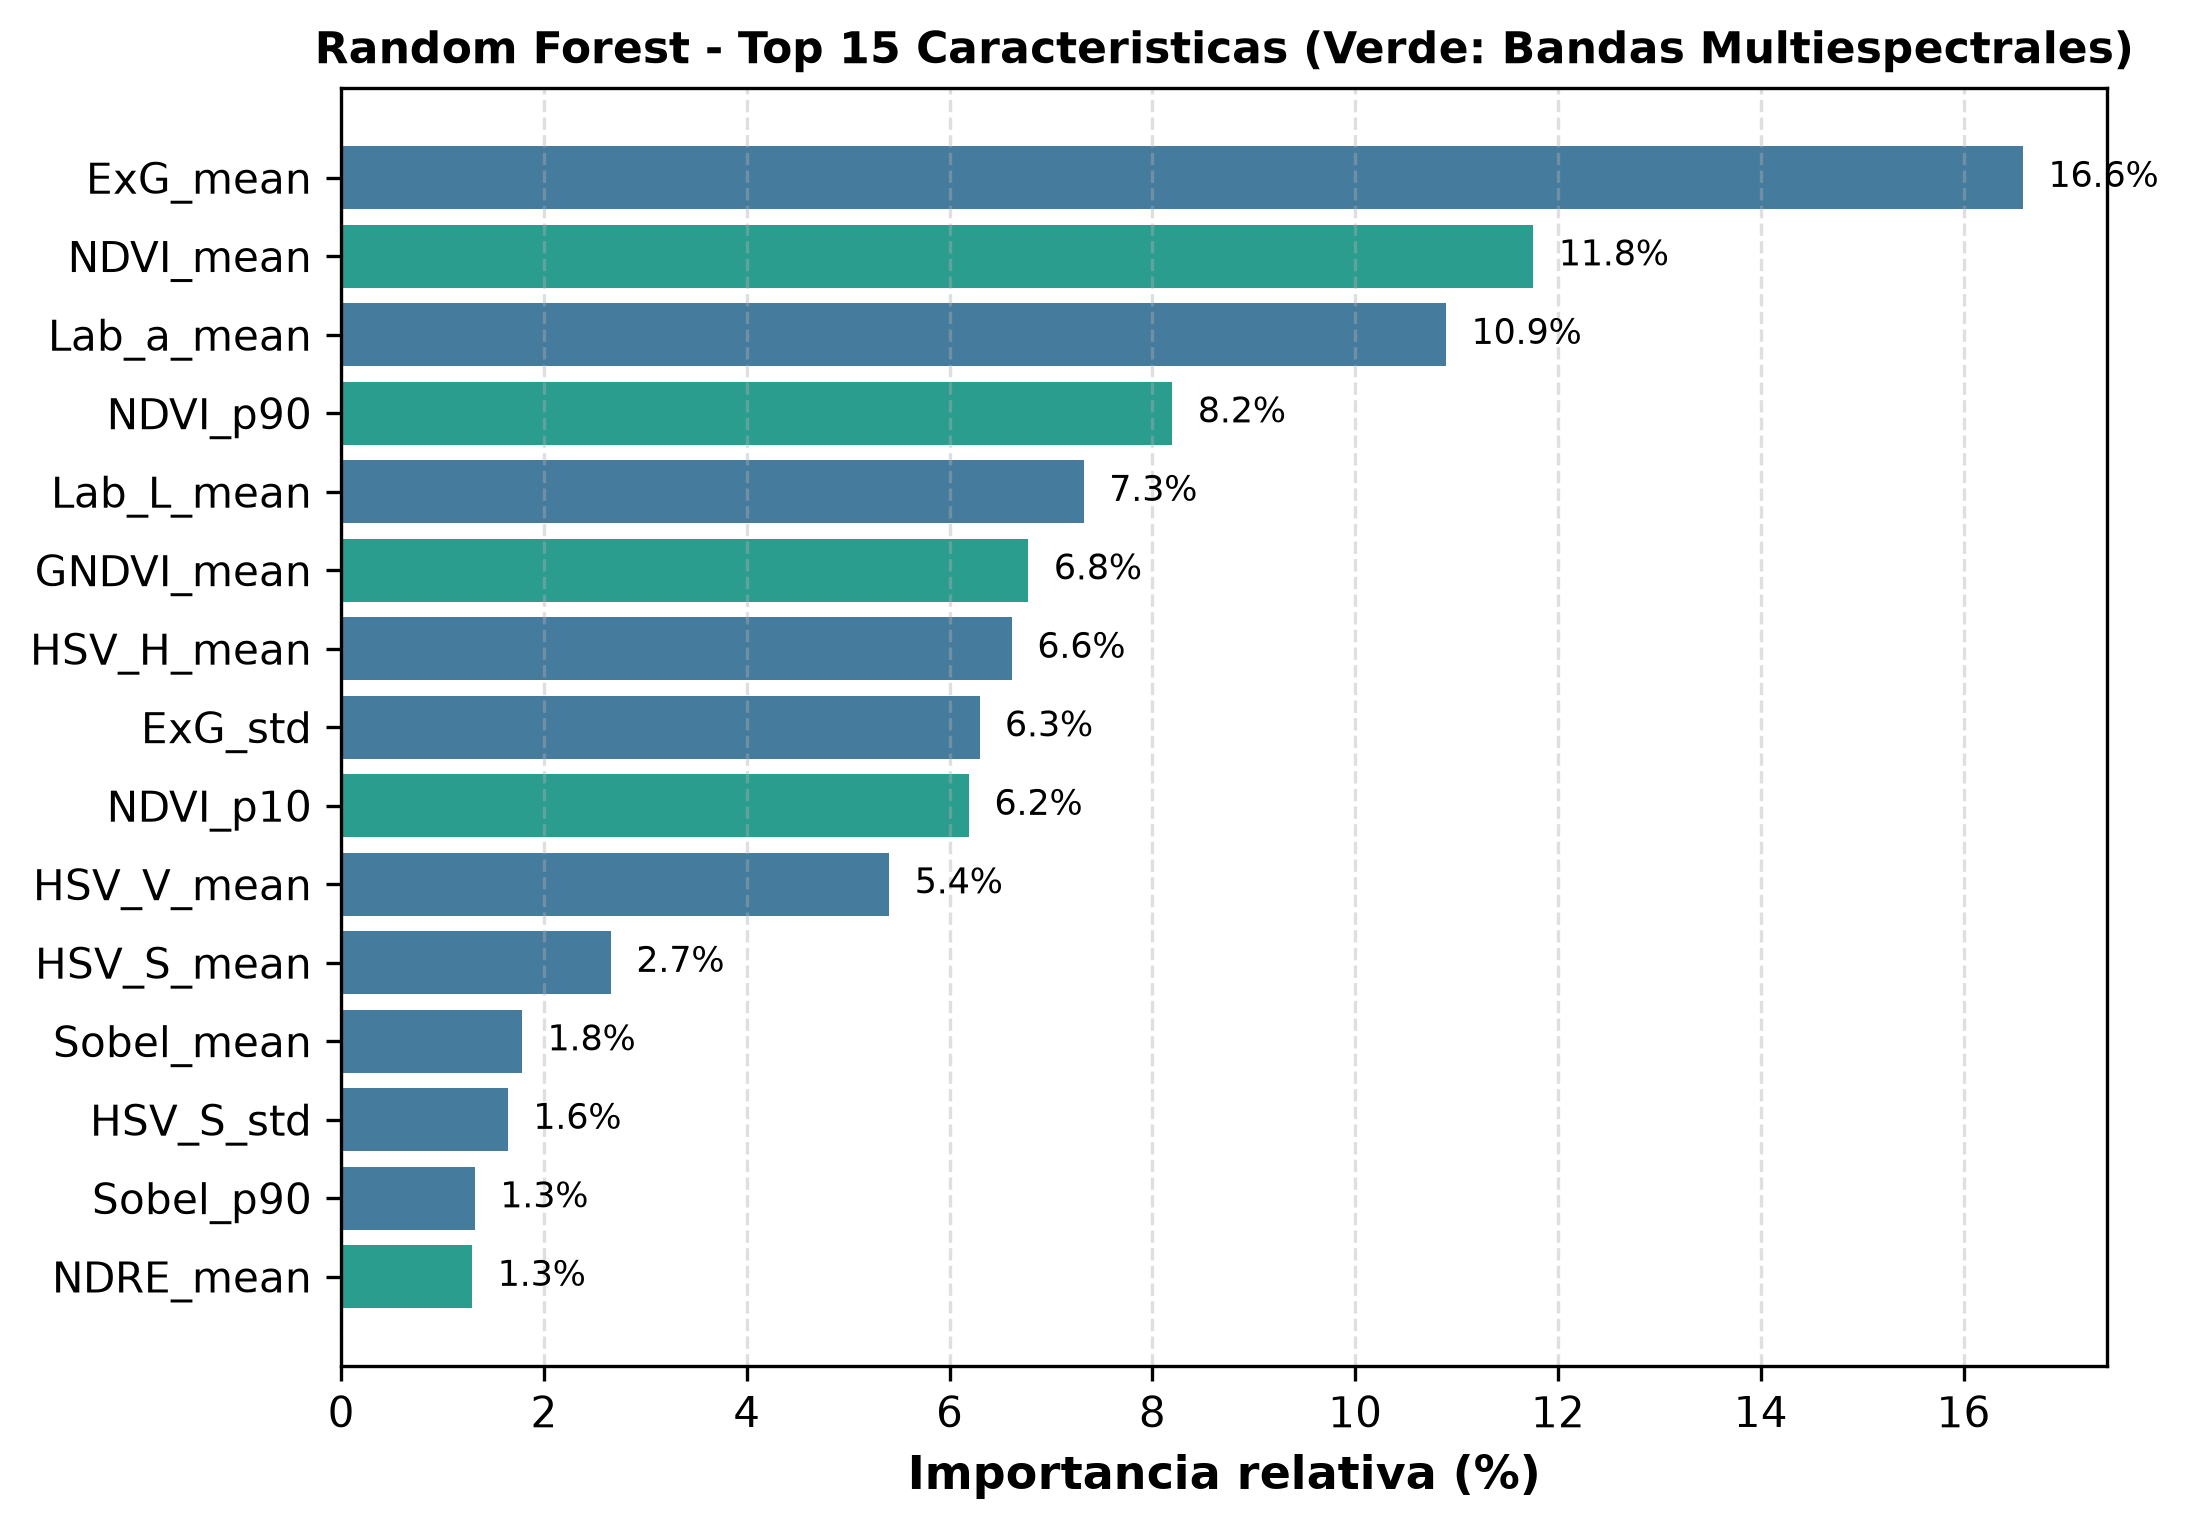
\includegraphics[width=\columnwidth]{figuras/fig3_importancia_rf.png}
\caption{Top 15 de características más relevantes en Random Forest. En verde se resaltan los índices derivados de bandas multiespectrales (NDVI, GNDVI, NDRE).}
\label{fig:imp_rf}
\end{figure}

\subsection{Desempeño de Segmentación Profunda (YOLO11n-seg)}
\guia{Redacta ~110 palabras analizando la Tabla~\ref{tab:yolo} y la Fig.~\ref{fig:cm_yolo}: explica que \texttt{YOLO11n-seg} opera únicamente con imágenes RGB (sin requerir sensor infrarrojo en inferencia) en $29.4\text{ ms}$ por parche en CPU. A nivel píxel alcanza $93.98\%$ de exactitud, $78.47\%$ de F1-macro y $66.55\%$ de mIoU, destacando en \texttt{vegetacion\_sana} ($95.22\%$ F1, $90.88\%$ IoU) y \texttt{suelo\_desnudo} ($99.64\%$ precisión). Comenta honestamente por qué \texttt{vegetacion\_seca} presenta menor recall ($50.77\%$) y mAP50 por instancia ($14.51\%$): la hojarasca y ramas secas bajo sombra son irregulares, fragmentadas y espectralmente ambiguas sin banda NIR.}

\begin{table}[!t]
\centering
\caption{Métricas de YOLO11n-seg (solo RGB) en el conjunto de prueba espacial (41 parches, 4 waypoints no vistos).}
\label{tab:yolo}
\resizebox{\columnwidth}{!}{%
\begin{tabular}{lccccc}
\toprule
\textbf{Clase} & \textbf{Prec. (Px)} & \textbf{Rec. (Px)} & \textbf{F1 (Px)} & \textbf{IoU (Px)} & \textbf{mAP50 (Inst.)} \\
\midrule
\texttt{vegetacion\_seca} & 0.838 & 0.508 & 0.632 & 0.462 & 0.145 \\
\texttt{vegetacion\_sana} & 0.948 & 0.957 & 0.952 & 0.909 & 0.724 \\
\texttt{suelo\_desnudo}   & 0.996 & 0.627 & 0.770 & 0.625 & 0.405 \\
\midrule
\textbf{Promedio / Global} & \textbf{0.927} & \textbf{0.697} & \textbf{0.785} & \textbf{0.666} & \textbf{0.424} \\
\bottomrule
\end{tabular}%
}
\end{table}

\begin{figure}[!t]
\centering
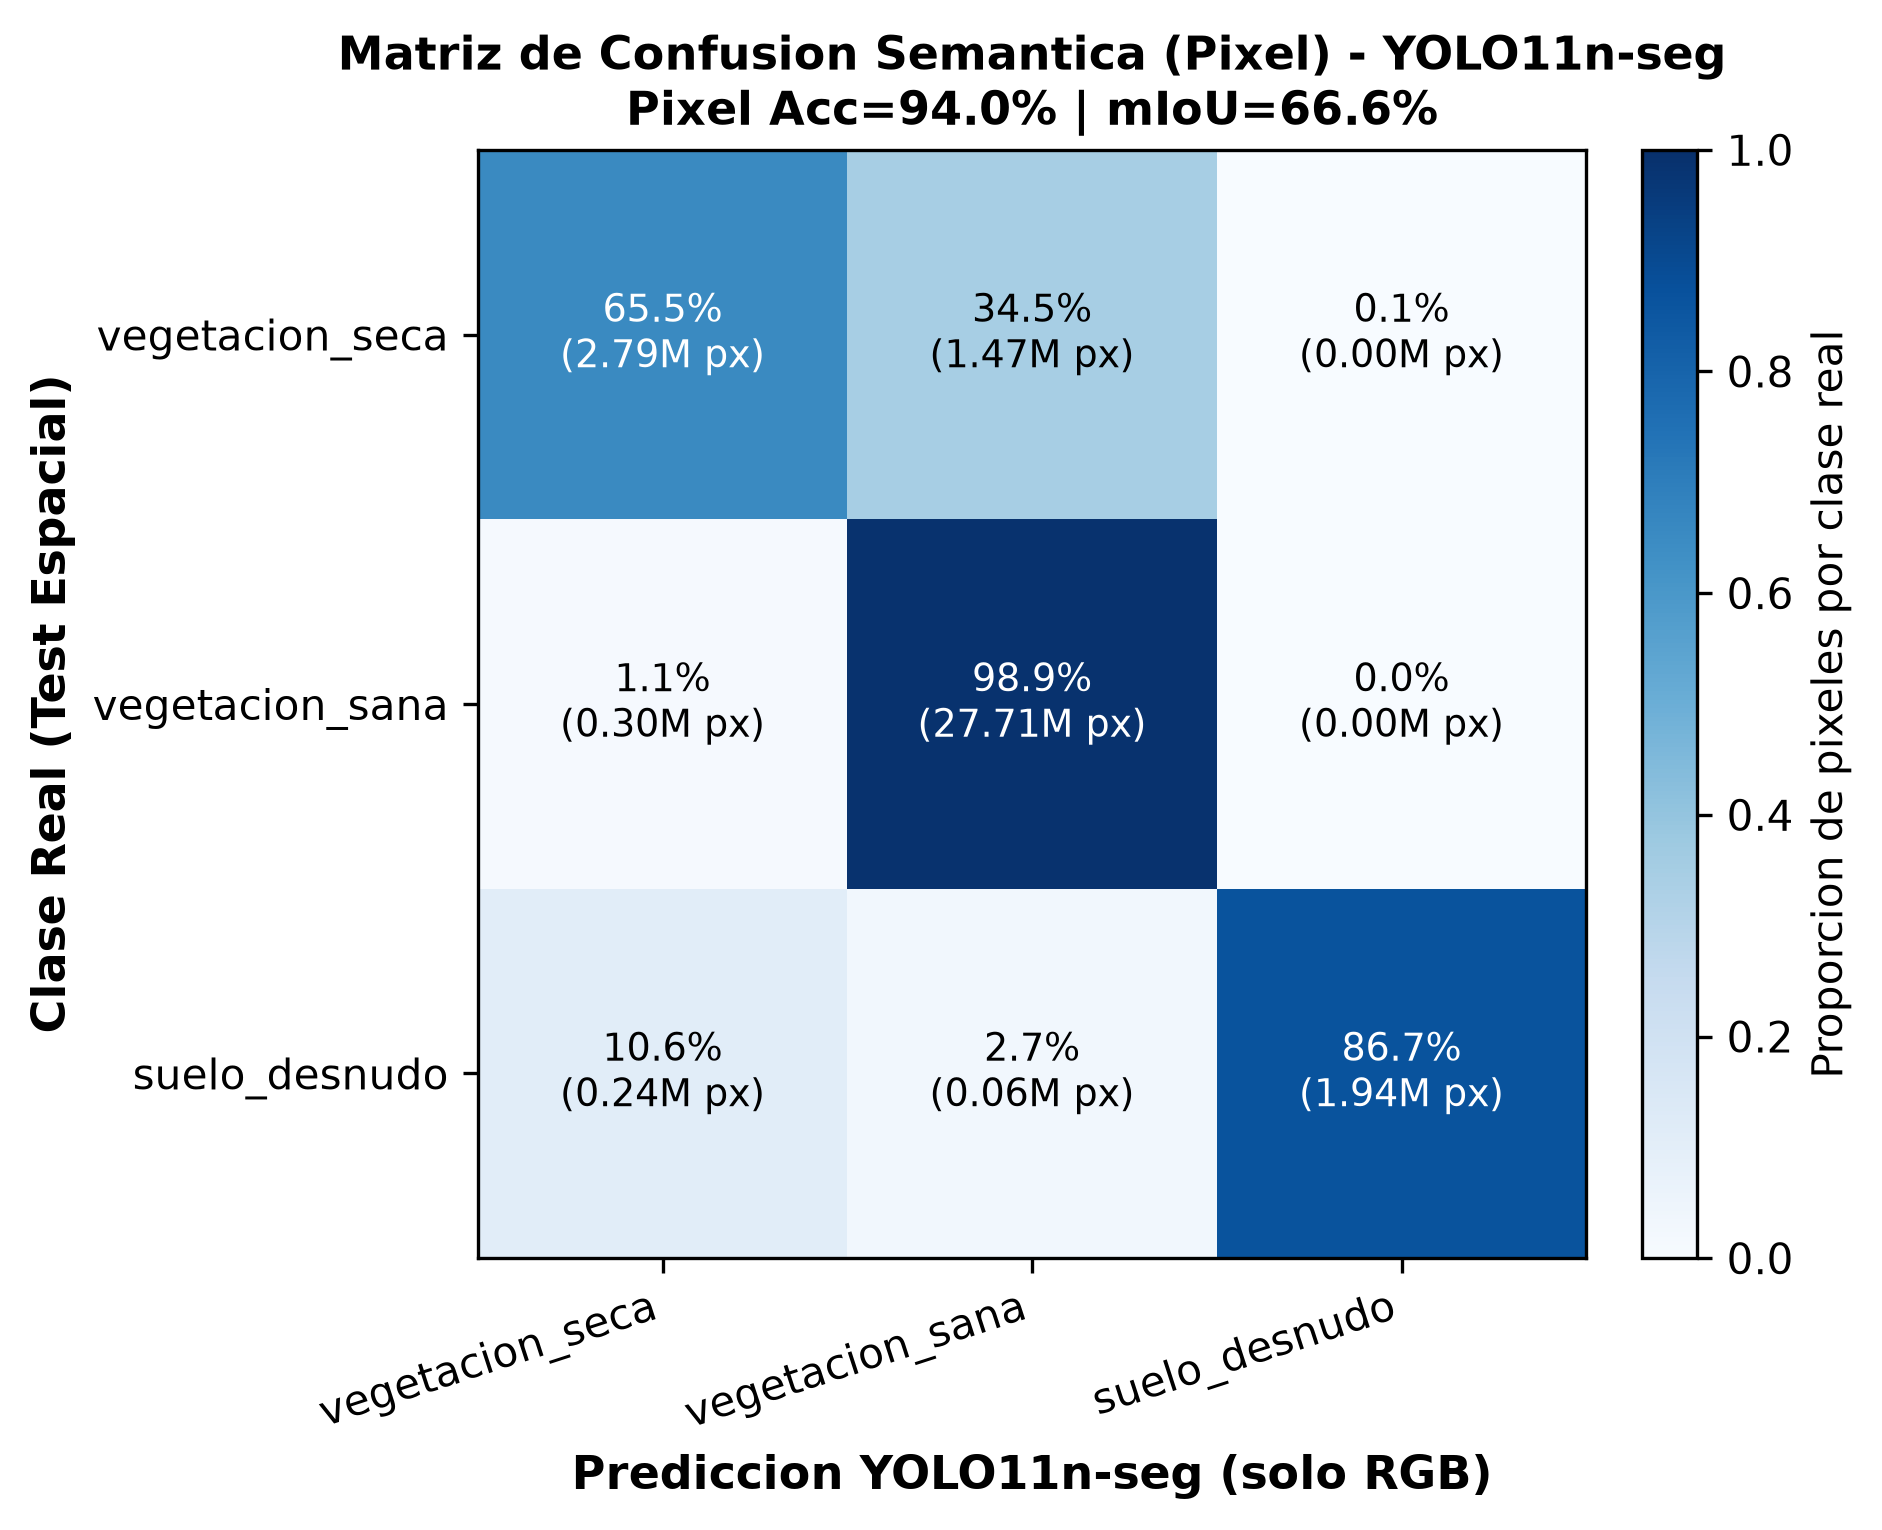
\includegraphics[width=0.92\columnwidth]{figuras/fig4_matriz_yolo.png}
\caption{Matriz de confusión semántica a nivel píxel de YOLO11n-seg sobre el subconjunto de prueba espacial.}
\label{fig:cm_yolo}
\end{figure}

\subsection{Mapas de Calor de Combustible y Variación Estacional}
\guia{Redacta ~120 palabras comentando las Figs.~\ref{fig:heat_wp01} y \ref{fig:heat_wp04} y la Tabla~\ref{tab:calor}: compara visualmente los 4 mapas de calor sobre las mismas fotografías aéreas completas de prueba. En el Waypoint 04 (2025) existe fuerte concordancia entre Random Forest ($24.2\%$), SVM ($23.4\%$) y YOLO11n-seg ($24.4\%$), clasificando la zona como riesgo moderado. Además, los 4 modelos capturan de forma consistente la reducción de biomasa seca entre marzo de 2025 y abril de 2026 debido a la brotación primaveral. Discute el compromiso operativo: los clasificadores multiespectrales logran mayor sensibilidad en claros pequeños sombreados, mientras YOLO11n-seg permite despliegue rápido en drones económicos con cámara RGB convencional ($1.5$--$2.7\text{ s}$ por fotografía de $20\text{ MP}$ en CPU).}

\begin{table}[!t]
\centering
\caption{Porcentaje de área detectada como \texttt{vegetacion\_seca} por modelo en las 8 capturas de prueba (2025 vs. 2026).}
\label{tab:calor}
\begin{tabular}{cccccc}
\toprule
\textbf{WP} & \textbf{Año} & \textbf{KNN (\%)} & \textbf{RF (\%)} & \textbf{SVM (\%)} & \textbf{YOLO (\%)} \\
\midrule
01 & 2025 & 23.3 & 20.0 & 17.6 & 13.3 \\
01 & 2026 & 18.1 &  9.7 & 13.0 &  1.3 \\
04 & 2025 & 28.6 & 24.2 & 23.4 & 24.4 \\
04 & 2026 & 24.7 & 16.2 & 16.4 &  2.8 \\
21 & 2025 & 10.7 &  6.1 &  5.1 &  2.9 \\
21 & 2026 &  9.0 &  4.4 &  4.5 &  1.2 \\
24 & 2025 & 11.5 &  8.1 &  7.6 &  5.4 \\
24 & 2026 &  7.4 &  2.5 &  3.5 &  0.3 \\
\bottomrule
\end{tabular}
\end{table}

\begin{figure*}[!t]
\centering
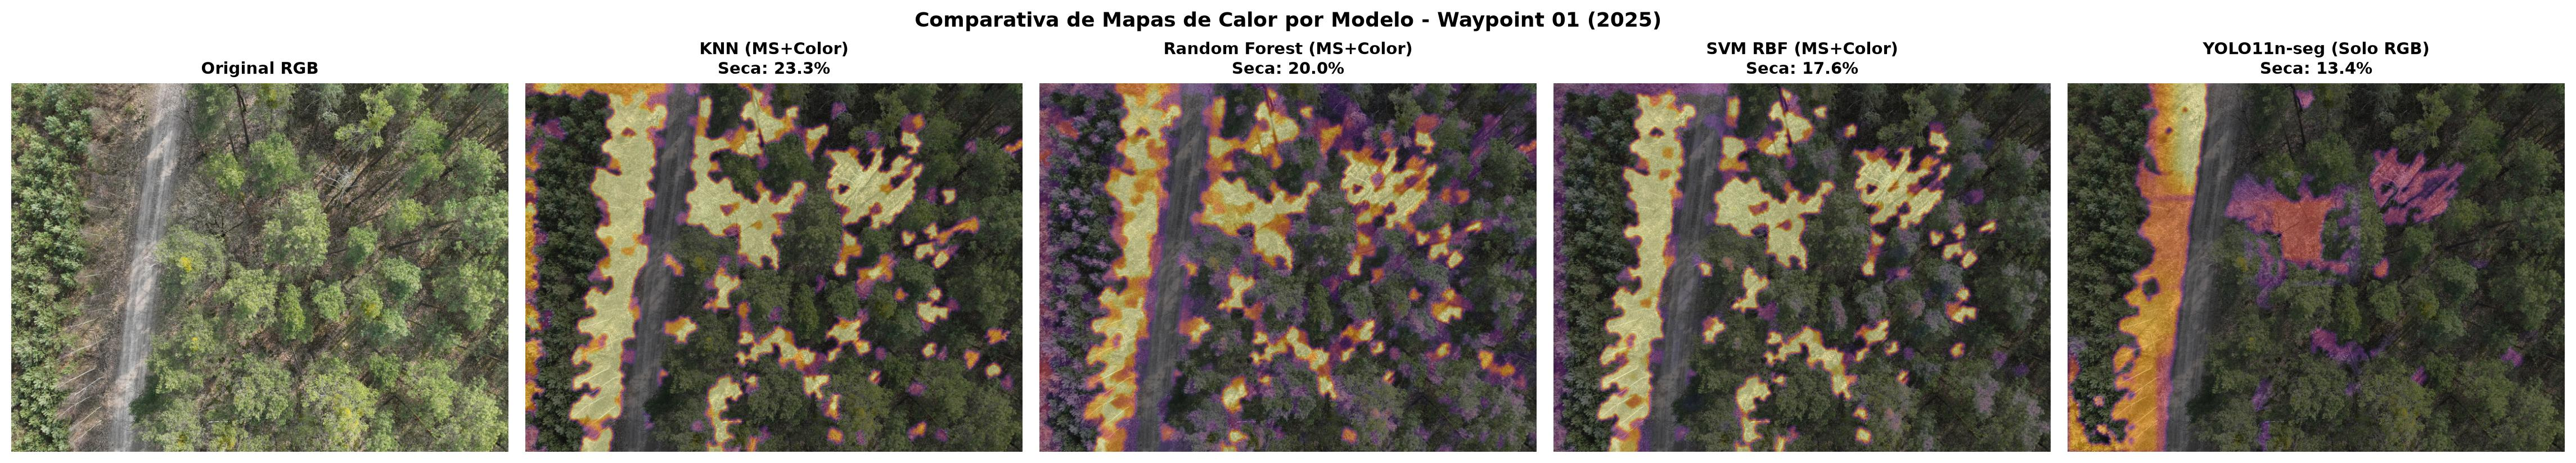
\includegraphics[width=0.98\textwidth]{figuras/fig5_mapas_calor_wp01.jpg}
\caption{Comparativa de mapas de calor de probabilidad de \texttt{vegetacion\_seca} en Waypoint 01 (2025, conjunto de prueba no visto): Original RGB, KNN, Random Forest, SVM RBF (multiespectral+color) y YOLO11n-seg (solo RGB).}
\label{fig:heat_wp01}
\end{figure*}

\begin{figure*}[!t]
\centering
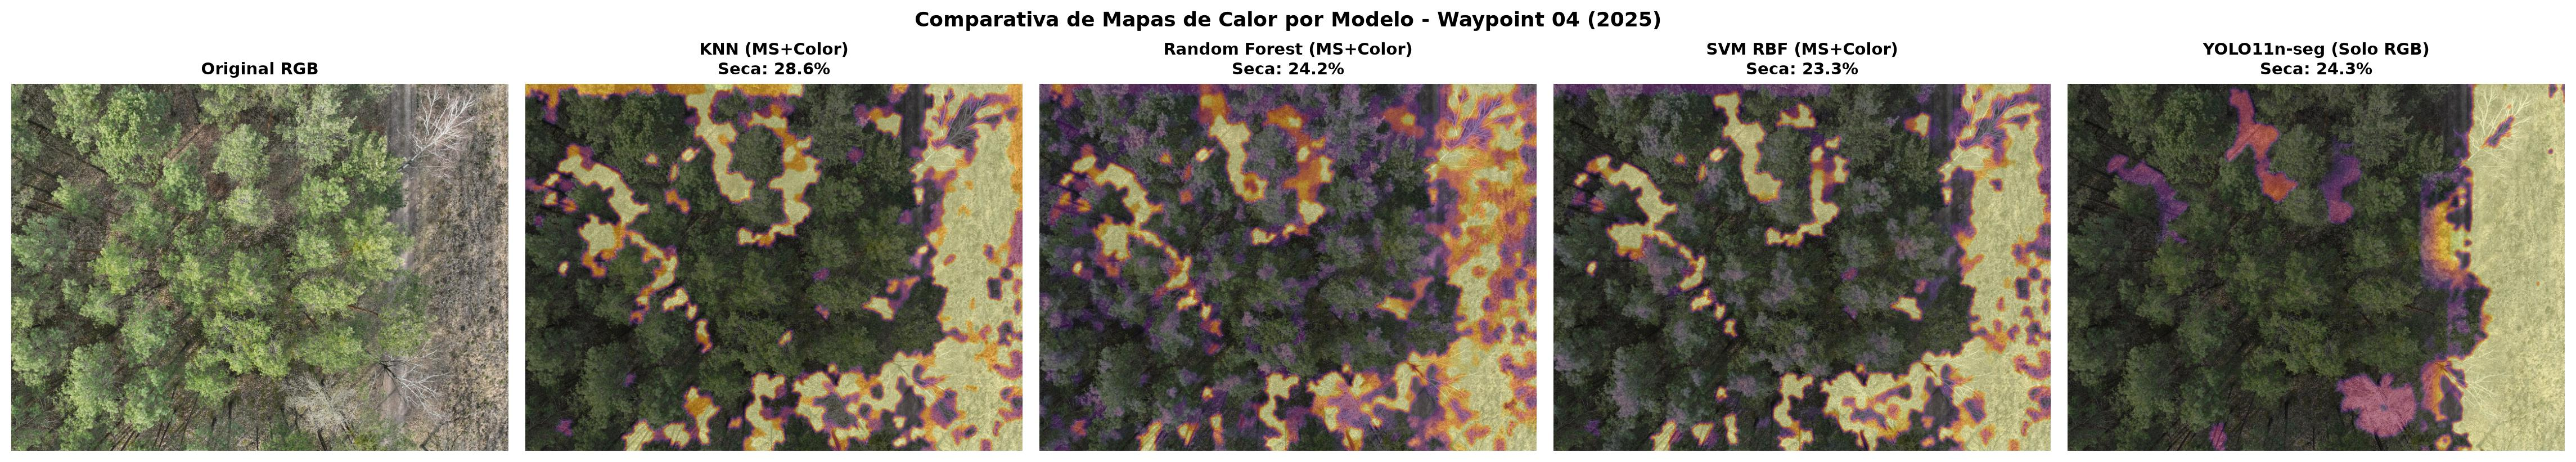
\includegraphics[width=0.98\textwidth]{figuras/fig6_mapas_calor_wp04.jpg}
\caption{Comparativa de mapas de calor en Waypoint 04 (2025, zona de riesgo moderado): concordancia espacial entre Random Forest ($24.2\%$), SVM ($23.3\%$) y YOLO11n-seg ($24.3\%$) sobre el claro seco adyacente al camino forestal.}
\label{fig:heat_wp04}
\end{figure*}

% =========================================================================
% V. CONCLUSIONES Y TRABAJO FUTURO
% =========================================================================
\section{Conclusiones y Trabajo Futuro}

\guia{Párrafo 1 (Síntesis de hallazgos, ~100 palabras): Resume con tus palabras las 3 conclusiones principales:
(1) la información multiespectral calibrada y el color superan ampliamente al descriptor HOG en escala de grises ($+36$ a $+50$ puntos de F1-macro en anotaciones manuales);
(2) la partición espacial por waypoint y la validación cruzada Zero-Shot ($91.0\%$ en RF) demuestran generalización real sobre zonas del bosque nunca vistas;
(3) \texttt{YOLO11n-seg} ofrece una alternativa viable solo con RGB ($94.0\%$ de exactitud a nivel píxel y procesamiento en $\sim 2\text{ s}$ por fotografía de 20 MP en CPU) para monitoreo preventivo ágil.}

\guia{Párrafo 2 (Limitaciones y trabajo futuro, ~80 palabras): Propone mejoras concretas derivadas de tus propios resultados: (a) entrenar arquitecturas de segmentación profunda con entrada de 4--5 canales (\texttt{RGB + NDVI + NDRE}) para elevar el recall en \texttt{vegetacion\_seca}; (b) ampliar el dataset a campañas de verano/sequía extrema y añadir diferenciación de especies caducifolias en reposo invernal; (c) integrar el modelo en un flujo de georreferenciación de ortomosaicos completos.}

% =========================================================================
% REFERENCIAS
% =========================================================================
\bibliographystyle{IEEEtran}
\bibliography{referencias}

\end{document}
